\section{Pronostic de l'état de santé des composants de stockage d'énergie}
% ============================================================
%  CHAPITRE — Section : Pronostic de l'état de santé des
%             composants de stockage d'énergie
%
%  Sous-section 1 : État de l'art & choix de la structure
%                   algorithmique
%
%  CITATIONS PLACEHOLDER à ajouter au .bib :
%    \cite{vetter_ageing_2005}        → J. Vetter et al., J. Power Sources, vol.147, 2005
%    \cite{dubau_review_2014}         → L. Dubau et al., WIREs Energy Env., vol.3, 2014
%    \cite{zhang_health_2023}         → C. Zhang et al., Renew. Sustain. Energy Rev., vol.182, 2023
%    \cite{kim_novel_2021}            → S. Kim et al., IEEE Trans. Ind. Electron., vol.68, 2021
%    \cite{ahwiadi_enhanced_2022}     → M. Ahwiadi & W. Wang, Measurement, vol.191, 2022
%    \cite{ao_pemfc_2021}             → Y. Ao et al., IEEE Trans. Transp. Electrif., vol.7, 2021
%    \cite{catelani_remaining_2021}   → M. Catelani et al., IEEE Trans. Instrum. Meas., vol.70, 2021
%    \cite{yue_degradation_2022}      → M. Yue et al., Control Eng. Practice, vol.118, 2022
%    \cite{zhang_accurate_2023}       → L. Zhang et al., Batteries, vol.9, 2023
%    \cite{wang_novel_2022}           → C. Wang et al., Int. J. Hydrogen Energy, vol.47, 2022
%    \cite{chen_transformer_2022}     → D. Chen et al., IEEE Access, vol.10, 2022
%    \cite{lv_transformer_2024}       → J. Lv et al., IEEE Trans. Transp. Electrif., vol.10, 2024
%    \cite{chandra_evaluation_2021}   → R. Chandra et al., IEEE Access, vol.9, 2021
%    \cite{hewamalage_recurrent_2021} → H. Hewamalage et al., Int. J. Forecasting, vol.37, 2021
%  Clés déjà présentes dans le .bib :
%    \cite{bressel_extended_2016}
%    \cite{papakonstantinou_degradation_2020}
%    \cite{noura_review_2020}
%    \cite{nguyen_comprehensive_2023}
% ============================================================
Les sections précédentes ont établi les définitions du SoH pour chacun des composants de stockage du micro-réseau, ainsi que les méthodes permettant de l'estimer en ligne à partir de mesures électriques. Cette estimation fournit une connaissance de l'état actuel de santé du système. Cette approche permettra d'adopter une approche réactive au vieillissement lors de la partie de gestion de l'énergie, présentée aux chapitres suivants. Cependant, une connaissance de l'évolution future du SoH ouvre la voie à une approche proactive, dans laquelle l'EMS peut anticiper les dégradations à venir et adapter sa stratégie en conséquence — par exemple en protégeant un composant dont la fin de vie approche. C'est l'objet du pronostic, qui vise à extrapoler les séries temporelles de SoH estimées vers le futur afin d'en déduire la durée de vie résiduelle (\textit{Remaining Useful Life}, ou RUL) des composants.

% ------------------------------------------------------------
\subsection{État de l'art \& choix de la structure algorithmique}
% ------------------------------------------------------------

Il existe plusieurs méthodes qui peuvent permettre d'extrapoler l'évolution de l'état de santé d'un composant de stockage en fonction des données passées. Les méthodes développées dans la littérature peuvent être regroupées en deux grandes familles : les approches basées sur des modèles physiques, et les approches basées sur les données.

% - - - - - - - - - - - - - - - - - - - - - - - - - - - - - -
\subsubsection{Méthodes basées modèle}
% - - - - - - - - - - - - - - - - - - - - - - - - - - - - - -

Les méthodes basées sur des modèles reposent sur une description mathématique du processus de dégradation du composant considéré. Elles sont généralement fondées sur des algorithmes de filtrage récursif (filtres particulaires, filtres de Kalman étendus ou non parfumés) qui propagent dans le temps un modèle de l'évolution du SoH afin d'en prédire la trajectoire future~\cite{kim_novel_2021}\cite{ahwiadi_enhanced_2022}. Pour les piles à combustible, des approches par filtre de Kalman dans le domaine fréquentiel ont également été proposées~\cite{ao_proton_2021}, et constituent une extension naturelle des méthodes de diagnostic présentées dans la section précédente~\cite{bressel_extended_2016}.

Ces méthodes présentent plusieurs avantages~: elles sont généralement rapides à exécuter, simples à implémenter, et leur comportement est interprétable physiquement. Leur principal inconvénient est leur dépendance forte au modèle de dégradation utilisé. Ce modèle doit être choisi \textit{a priori} et est spécifique à chaque type de composant et à chaque profil d'utilisation. Pour les batteries lithium-ion, par exemple, les modèles de dégradation disponibles dans la littérature sont nombreux et bien validés~\cite{vetter_ageing_2005}\cite{noura_review_2020}, mais ils ne se transposent pas directement aux composants hydrogène, dont les mécanismes de vieillissement sont différents~\cite{dubau_review_2014}\cite{papakonstantinou_degradation_2020}. Cette spécificité limite la généralité des approches basées modèle dans le contexte d'un micro-réseau avec stockage hybride, où batteries, piles à combustible et électrolyseurs coexistent.

% - - - - - - - - - - - - - - - - - - - - - - - - - - - - - -
\subsubsection{Méthodes basées données}
% - - - - - - - - - - - - - - - - - - - - - - - - - - - - - -

Les méthodes orientées données surmontent cette limitation en apprenant directement les tendances de dégradation à partir des séries temporelles historiques de SoH, sans hypothèse sur la forme du modèle de vieillissement sous-jacent. Elles s'appliquent indifféremment à tout composant pour lequel une série temporelle de SoH est disponible, ce qui en fait des approches naturellement polyvalentes dans un contexte multi-technologies.

Les réseaux de neurones récurrents (\textit{Recurrent Neural Networks}, ou RNN) sont les structures algorithmiques de référence pour la gestion des séries temporeles. Parmi les architectures de RNNs, trois approches sont principalement représentées dans la littérature pour le pronostic de composants de stockage~:

\begin{itemize}
    \item Les \textit{Echo State Networks}(ESN) constituent l'approche la plus légère d'un point de vue informatique. Leurs poids internes sont fixés aléatoirement et seule la couche de sortie est entraînée, ce qui les rend rapides à optimiser. En contrepartie, leurs performances sont limitées pour les tendances complexes et les dépendances temporelles longues~\cite{catelani_remaining_2021}\cite{yue_degradation_2022}.

    \item Les réseaux \textit{Long Short-Term Memory} (LSTM) représentent un compromis plus avancé. L'implémentation explicite d'une mémoire à long-terme leur permet de conserver sélectivement de l'information sur de plus longues périodes. Cela résout également le problème de disparition du gradient des RNNs traditionnels. Ils ont été appliqués avec succès au pronostic de batteries~\cite{zhang_accurate_2023} et de piles à combustible~\cite{wang_novel_2022}, et constituent aujourd'hui la technologie la plus utilisée et la mieux validée pour ces applications.

    \item Les architectures \textit{Transformer}, basées sur des mécanismes d'attention, représentent la voie la plus récente et la plus puissante. Elles permettent de corréler des dépendances à très longue portée dans les séries temporelles et ont été appliquées au pronostic de batteries~\cite{chen_transformer_2022} et de piles à combustible~\cite{lv_transformer_2024}. Leur complexité algorithmique et leurs besoins en données d'entraînement restent cependant nettement supérieurs à ceux des LSTM, et leur maturité relative pour les applications de pronostic de composants de stockage est encore moindre~\cite{chandra_evaluation_2021}\cite{hewamalage_recurrent_2021}.
\end{itemize}

Un résumé des méthodes de pronostic d'état de santé est donné dans le tableau \ref{tab:state_of_art_prognosis} : 

\begin{table}[h]
\centering
\caption{Synthèse des méthodes de pronostic et d'extrapolation du SoH\vspace{0.4cm}}
\begin{tabular}{M{2.5cm} M{4.2cm} M{3.1cm} M{3.8cm} }
\hline
\textbf{Familles} & \textbf{Méthodes \& Références} & \textbf{Avantages} & \textbf{Inconvénients} \\
\hline \hline
\multirow{3}{2.5cm}{\centering Méthodes basées modèle} 
& \vspace{0.15cm} Filtrage récursif (EKF, UKF, PF) \cite{kim_novel_2021, ahwiadi_enhanced_2022} \vspace{0.15cm} & \multirow{1}{2.7cm}{\centering Rapides à exécuter, interprétables physiquement} & \multirow{2}{3.2cm}{\centering Dépendance forte au modèle choisi \textit{a priori}, manque de généralité} \\
\cline{2-2}
& \vspace{0.15cm} Filtrage dans le domaine fréquentiel \cite{ao_proton_2021, bressel_extended_2016} \vspace{0.15cm} &  &  \\
\hline
\multirow{5}{2.5cm}{\centering Méthodes basées données (RNN)} 
& \vspace{0.15cm} Echo State Networks (ESN) \cite{catelani_remaining_2021, yue_degradation_2022} \vspace{0.15cm} & \multirow{6}{2.7cm}{\centering Polyvalence (multi-technologies), pas d'hypothèse de modèle, capture des tendances complexes} & Performances limitées sur les dépendances longues \vspace{0cm} \\
\cline{2-2} \cline{4-4}
& \vspace{0.15cm} Long Short-Term Memory (LSTM)  \cite{zhang_accurate_2023, wang_novel_2022} \vspace{0.15cm} &  & Compromis calcul/performance \vspace{0.1cm}\\
\cline{2-2} \cline{4-4}
& \vspace{0.15cm} Architectures Transformer \cite{chen_transformer_2022, lv_transformer_2024} \vspace{0.15cm} &  & Complexité élevée, plus faible maturité \vspace{0.1cm} \\
\hline
\end{tabular}
\label{tab:state_of_art_prognosis}
\end{table}
\FloatBarrier

Au regard de ces éléments, l'architecture LSTM est retenue comme le meilleur compromis entre performance prédictive, polyvalence et maturité technologique~\cite{chandra_evaluation_2021}. Elle offre en outre l'avantage décisif d'être directement applicable à tout type de série temporelle de SoH — qu'il s'agisse de la capacité d'une batterie, du paramètre $\alpha$ d'une pile à combustible ou d'un électrolyseur — permettant ainsi une approche unifiée pour l'ensemble des composants du micro-réseau hybride. L'algorithme et son application sont détaillés dans les sous-sections suivantes.

\subsection{Définition du \textit{Remaining Useful Life}}
% ============================================================
%  CHAPITRE — Section : Pronostic de l'état de santé des
%             composants de stockage d'énergie
%
%  Sous-section 2 : Définition du Remaining Useful Life (RUL)
%
%  CITATIONS PLACEHOLDER à ajouter au .bib :
%    \cite{lei_machinery_2018}     → Y. Lei et al., Mech. Syst. Signal Process., vol.104, 2018
%                                    DOI: 10.1016/j.ymssp.2017.11.016
%    \cite{wang_novel_2021}        → P. Wang et al., Int. J. Hydrogen Energy, vol.46, 2021
%                                    DOI: 10.1016/j.ijhydene.2021.07.004
%  Clés déjà présentes dans le .bib :
%    \cite{noura_review_2020}
%    \cite{papakonstantinou_degradation_2020}
%    \cite{bressel_extended_2016}
% ============================================================
Le pronostic d'un composant a notamment pour finalité de fournir une estimation de sa durée de vie résiduelle, communément désignée par le RUL. Le RUL est défini comme la durée de fonctionnement restante avant que le composant n'atteigne son critère de fin de vie. Il constitue une grandeur opérationnelle directement exploitable par l'opérateur du système ou par une EMS proactive, en permettant d'anticiper les contraintes physiques futures et les décisions de maintenance.

Formellement, si l'on note $t_{\text{now}}$ l'instant courant et $t_{\text{EoL}}$ l'instant auquel le SoH prédit atteindra le seuil de fin de vie $\text{SoH}_{\text{EoL}}$, le RUL s'écrit~:

\begin{equation}
    \text{RUL}(t_{\text{now}}) = t_{\text{EoL}} - t_{\text{now}}
    \label{eq:rul_definition}
\end{equation}

Les seuils de fin de vie $\text{SoH}_{\text{EoL}}$ sont fixés selon les définitions introduites aux sections précédentes~: une perte de capacité de 40\,\% pour la batterie, une perte de puissance de 10\,\% pour la PEMFC, et une augmentation de 10\,\% de la puissance consommée pour le PEMWE. 
Le calcul du RUL à partir d'une prédiction de SoH repose sur l'intersection entre la trajectoire projetée et le seuil de fin de vie, illustrée schématiquement à la Figure~\ref{fig:rul_concept}. Cette opération est réalisée a posteriori, une fois la prédiction de la série temporelle future de SoH obtenue par le réseau LSTM.

\begin{figure}[h!]
    \centering
    % placeholder — schéma conceptuel du RUL : trajectoire SoH projetée,
    % seuil EoL, instant courant, et RUL correspondant
    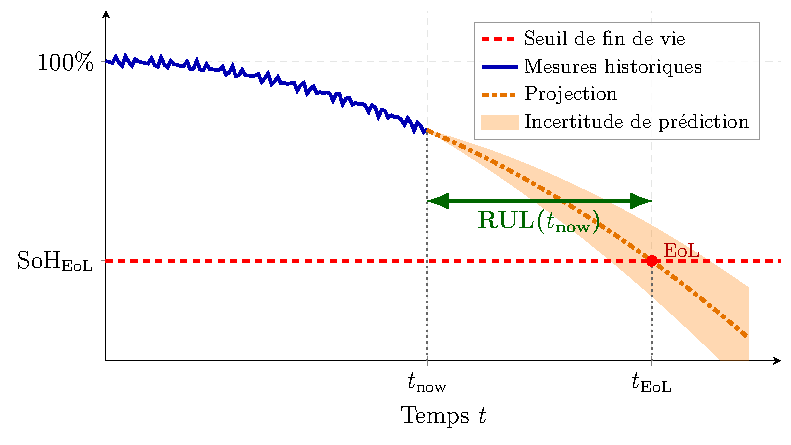
\includegraphics[width=\linewidth]{Chapitre 1/Prono/Figures/rul.pdf}
    \caption{Représentation schématique du calcul du RUL à partir de la projection du SoH : intersection entre la trajectoire projetée et le seuil de fin de vie.}
    \label{fig:rul_concept}
\end{figure}
\FloatBarrier

Il est important de souligner que le RUL ainsi calculé n'est pas une grandeur déterministe mais une estimation probabiliste, dont la précision dépend directement de la qualité de la prédiction de SoH et de l'horizon sur lequel elle est réalisée. L'incertitude sur le RUL est ici propagée à partir de l'incertitude sur la prédiction de SoH, qui sera introduite à la sous-section~\ref{subsec:mcdropout}. 

% ============================================================
%
%  Sous-section 3 : Principe du réseau LSTM
%
%  CITATIONS PLACEHOLDER à ajouter au .bib :
%    \cite{hochreiter_lstm_1997}      → S. Hochreiter & J. Schmidhuber, Neural Computation,
%                                       vol.9, no.8, pp.1735-1780, 1997
%                                       DOI: 10.1162/neco.1997.9.8.1735
%    \cite{hewamalage_recurrent_2021} → H. Hewamalage et al., Int. J. Forecasting, vol.37, 2021
%                                       DOI: 10.1016/j.ijforecast.2020.06.008
%                                       (déjà listé en ss1 — même clé)
%    \cite{chandra_evaluation_2021}   → R. Chandra et al., IEEE Access, vol.9, 2021
%                                       DOI: 10.1109/ACCESS.2021.3085871
%                                       (déjà listé en ss1 — même clé)
%    \cite{wang_novel_2022}           → C. Wang et al., Int. J. Hydrogen Energy, vol.47, 2022
%                                       DOI: 10.1016/j.ijhydene.2021.11.204
%                                       (déjà listé en ss1 — même clé)
% ============================================================

\subsection{Principe du réseau LSTM}

Les réseaux de neurones LSTM ont été introduits par Hochreiter et Schmidhuber~\cite{hochreiter_long_1997} pour pallier la limitation fondamentale des réseaux de neurones récurrents classiques~: le problème de disparition du gradient. Dans un RNN standard, le gradient de l'erreur est rétropropagé à travers le temps lors de l'entraînement ; lorsque les séquences sont longues, ce gradient tend à s'annuler exponentiellement, empêchant le réseau d'apprendre des dépendances temporelles éloignées. Les LSTM résolvent ce problème grâce à un mécanisme de mémoire explicite, structuré autour de portes (\textit{gates}) qui régulent sélectivement le flux d'information entre les pas de temps.

\paragraph{Architecture d'un réseau LSTM.}\hfill \\
Une cellule LSTM maintient deux états internes entre pas de temps successifs~: l'état de cellule $c^{\langle t \rangle}$, qui constitue la mémoire à long terme du réseau, et l'état caché $h^{\langle t \rangle}$, qui représente la mémoire à court terme. À chaque pas de temps $t$, ces deux états interagissent avec le vecteur d'entrée $x^{\langle t \rangle}$ au travers de trois portes, dont le fonctionnement est illustré à la Figure~\ref{fig:lstm_cell}~:

\begin{itemize}
    \item La porte d'oubli (\textit{forget gate}) $f^{\langle t \rangle}$ détermine quelle fraction de l'état de cellule précédent $c^{\langle t-1 \rangle}$ doit être conservée. Elle produit un vecteur de valeurs comprises entre 0 et 1 via une activation sigmoïde~:
    \begin{equation}
        f^{\langle t \rangle} = \sigma\!\left(W_f \left[h^{\langle t-1 \rangle},\, x^{\langle t \rangle}\right] + b_f\right)
        \label{eq:lstm_forget}
    \end{equation}

    \item La porte d'entrée (\textit{input gate}) $i^{\langle t \rangle}$ et la fonction d'activation $\tilde{c}^{\langle t \rangle}$ déterminent quelle nouvelle information est ajoutée à l'état de cellule~:
    \begin{equation}
        i^{\langle t \rangle} = \sigma\!\left(W_i \left[h^{\langle t-1 \rangle},\, x^{\langle t \rangle}\right] + b_i\right)
        \label{eq:lstm_input}
    \end{equation}
    \begin{equation}
        \tilde{c}^{\langle t \rangle} = \tanh\!\left(W_c \left[h^{\langle t-1 \rangle},\, x^{\langle t \rangle}\right] + b_c\right)
        \label{eq:lstm_candidate}
    \end{equation}

    \item La porte de sortie (\textit{output gate}) $o^{\langle t \rangle}$ filtre l'état de cellule mis à jour pour produire l'état caché de sortie $h^{\langle t \rangle}$~:
    \begin{equation}
        o^{\langle t \rangle} = \sigma\!\left(W_o \left[h^{\langle t-1 \rangle},\, x^{\langle t \rangle}\right] + b_o\right)
        \label{eq:lstm_output_gate}
    \end{equation}
\end{itemize}

Ces trois portes permettent de calculer les mises à jour des états internes~:
\begin{align}
    c^{\langle t \rangle} &= f^{\langle t \rangle} \odot c^{\langle t-1 \rangle} + i^{\langle t \rangle} \odot \tilde{c}^{\langle t \rangle}
    \label{eq:lstm_cell_update} \\
    h^{\langle t \rangle} &= o^{\langle t \rangle} \odot \tanh\!\left(c^{\langle t \rangle}\right)
    \label{eq:lstm_hidden_update}
\end{align}

où $\odot$ désigne le produit élément par élément (\textit{Hadamard product}), $W_f$, $W_i$, $W_c$, $W_o$ sont les matrices de poids apprenables, et $b_f$, $b_i$, $b_c$, $b_o$ les biais associés. Le vecteur de sortie $h^{\langle t \rangle}$ est à la fois transmis à la couche suivante du réseau et renvoyé à la même cellule au pas de temps suivant.

\begin{figure}[h!]
    \centering
    % placeholder — illustration d'une cellule LSTM avec ses trois portes,
    % ses deux états (cell et hidden) et les flux d'information
    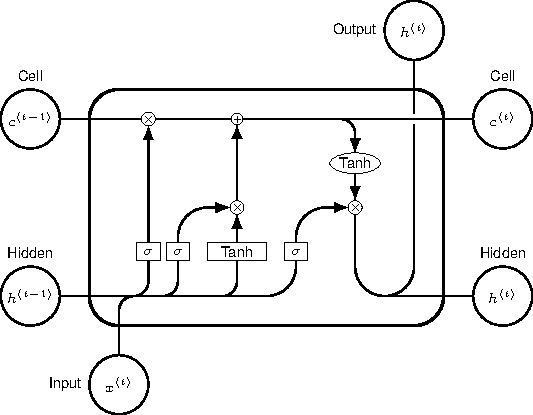
\includegraphics[width=0.85\linewidth]{Chapitre 1/Prono/Figures/lstm_cell.pdf}
    \caption{Illustration d'une cellule LSTM~: les états de cellule $c^{\langle t \rangle}$ (mémoire long terme) et caché $h^{\langle t \rangle}$ (mémoire court terme) interagissent avec l'entrée $x^{\langle t \rangle}$ via les trois portes d'oubli, d'entrée et de sortie.}
    \label{fig:lstm_cell}
\end{figure}
\FloatBarrier

Dans ce travail, l'architecture retenue consiste en une seule couche LSTM de $U$ unités, suivie d'une couche de régularisation par \textit{dropout} (taux $p$) et d'une couche dense de sortie à une unité. Cette architecture compacte s'avère suffisante pour capturer la dynamique de dégradation monotone qui caractérise les séries de SoH étudiées, tout en limitant le risque de sur-apprentissage sur des séries d'une longueur modérée~\cite{hewamalage_recurrent_2021}.


% ============================================================
%  CHAPITRE — Section : Pronostic de l'état de santé des
%             composants de stockage d'énergie
%
%  Sous-section 4 : Méthode & gestion des données
%    \subsubsection{Traitement des données brutes & construction
%                   des ensembles de données}
%    \subsubsection{Hyperparamètres}
%
%  CITATIONS PLACEHOLDER à ajouter au .bib :
%    \cite{goodfellow_deep_2016}   → I. Goodfellow et al., Deep Learning,
%                                    MIT Press, 2016. ISBN: 978-0262035613
%    \cite{srivastava_dropout_2014}→ N. Srivastava et al., J. Mach. Learn. Res.,
%                                    vol.15, pp.1929-1958, 2014
%    \cite{kingma_adam_2015}       → D.P. Kingma & J. Ba, ICLR 2015,
%                                    arXiv:1412.6980
%  Clés déjà présentes dans le .bib :
%    \cite{papakonstantinou_degradation_2020}
%    \cite{noura_review_2020}
% ============================================================

\subsection{Méthode \& gestion des données}

La performance d'un réseau LSTM pour le pronostic dépend de façon critique de la qualité et de la structure des données d'entraînement, ainsi que du choix des hyperparamètres qui gouvernent l'architecture et l'apprentissage. Cette sous-section décrit successivement la procédure de traitement des données brutes et de construction des ensembles d'entraînement, de validation et de test, puis les choix d'hyperparamètres retenus.

% - - - - - - - - - - - - - - - - - - - - - - - - - - - - - -
\subsubsection{Traitement des données brutes \& construction des ensembles de données}
% - - - - - - - - - - - - - - - - - - - - - - - - - - - - - -

\paragraph{Source des données.}\hfill \\
Les données qui sont traitées par le réseau pour le pronostic sont des séries temporelles de SoH. Pour ce chapitre, les données utilisées pour l'entraînement et la validation du réseau LSTM sont des évolutions des états de santé issus de la simulation du micro-réseau sur un horizon de quinze ans, telle qu'elle sera décrite au chapitre suivant. Il est considéré que, à chaque pas de temps de simulation (un jour ici), les méthodes d'estimation décrites précédemment fournissent des valeurs d'états de santé pour chacun des composants du stockage. Ces séries temporelles constituent le signal brut d'entrée du réseau LSTM.
Dans le cadre de cette thèse, les données de vieillissement ne sont pas issues de mesures expérimentales sur le micro-réseau réel de La Réunion, mais de la simulation. Cette approche suppose que le modèle de simulation reproduit fidèlement les tendances de dégradation réelles.

\paragraph{Normalisation.}\hfill \\
Avant tout traitement, les séries temporelles de SoH sont normalisées dans l'intervalle $[0, 1]$ afin de garantir une stabilité numérique lors de l'entraînement et de faciliter la convergence du réseau~\cite{heaton_ian_2018}. La normalisation est effectuée par mise à l'échelle min-max~:

\begin{equation}
    \hat{s}(t) = \frac{s(t) - s_{\min}}{s_{\max} - s_{\min}}
    \label{eq:normalisation}
\end{equation}

où $s(t)$ est la valeur brute du SoH à l'instant $t$, et $s_{\min}$, $s_{\max}$ sont respectivement la valeur minimale et maximale observées sur l'ensemble de la série d'entraînement. Les valeurs de $s_{\min}$ et $s_{\max}$ sont calculées sur l'ensemble d'entraînement uniquement et appliquées à l'ensemble de test, afin d'éviter toute fuite d'information (\textit{data leakage}) entre les deux ensembles.

\paragraph{Séquençage des données.}\hfill \\
Un réseau LSTM travaille sur des séquences d'entrée de longueur fixe. Le problème de pronostic est donc formulé comme suit~: étant donné une fenêtre glissante de $T$ pas de temps consécutifs de SoH normalisé, le réseau prédit le pas de temps suivants. L'application successive de ce réseau sur $H$ fenêtres glissantes successives permet ainsi de faire une prédiction à $H$ pas de temps. Le paramètre $T$ est appelé la taille de la séquence et $H$ l'horizon de prédiction. Ce séquençage est illustré à la Figure~\ref{fig:sequencing}.

\begin{figure}[h!]
    \centering
    % placeholder — illustration du séquençage par fenêtre glissante :
    % fenêtre d'entrée L, horizon de prédiction H, décalage d'un pas
    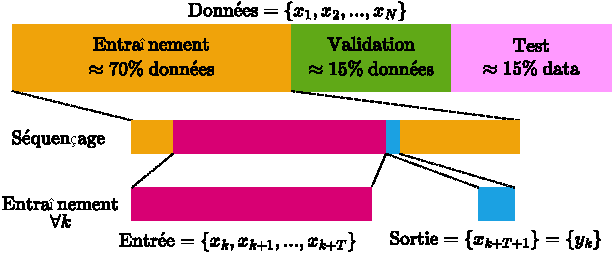
\includegraphics[width=\linewidth]{Chapitre 1/Prono/Figures/data_sequencing.pdf}
    \caption{Principe du séquençage par fenêtre glissante pour la construction des ensembles de données~: chaque échantillon d'entraînement est constitué d'une fenêtre d'entrée de longueur $T$}
    \label{fig:sequencing}
\end{figure}
\FloatBarrier

À partir d'une série temporelle d'entraînement de longueur totale $N$, cette procédure génère $N - T$ paires (entrée, cible), formant l'ensemble de données complet. La fenêtre glisse d'un pas à la fois, ce qui garantit une couverture dense de l'ensemble de la trajectoire de dégradation et maximise le nombre d'exemples d'entraînement disponibles. Lorsque le modèle atteint les ensembles de validation ou de test, il effectue par la suite des prédictions récursives, c'est-à-dire qu'il utilise ses propres données prédites à un instant donné pour construire la séquence de l'instant suivant et ainsi de suite. Cela garantit que la prédiction fait à un instant donné n'utilise que les mesures qui ont été effectuées jusqu'à cet instant.

\paragraph{Construction des ensembles d'entraînement, validation et test}\hfill \\
L'ensemble de données est divisé en un ensemble d'entraînement, un ensemble de validation et un ensemble de test selon une règle de séparation temporelle stricte~: les données des premières fractions (70\%) de la série temporelle constituent l'ensemble d'entraînement, les (15\%) suivants constituent l'ensemble de validation, et la portion finale (15\%) est réservée pour le test. L'objectif est alors de trouver une combinaison d'hyperparamètres qui minimisera la fonction de coût sur l'ensemble de validation, entre autres afin de prévenir l'\textit{overfitting}. Une fois une combinaison satisfaisante obtenue, l'ensemble de test servira à avoir une vue sur les performances de prédiction de l'algorithme.

% - - - - - - - - - - - - - - - - - - - - - - - - - - - - - -
\subsubsection{Hyperparamètres}
% - - - - - - - - - - - - - - - - - - - - - - - - - - - - - -

Les hyperparamètres du réseau LSTM sont les paramètres qui ne sont pas appris lors de l'entraînement mais fixés avant celui-ci. Ils gouvernent à la fois l'architecture du réseau (nombre de couches, \textit{dropout}) et la procédure d'apprentissage (taux d'apprentissage, nombre d'epochs), ainsi que d'autres paramètres sur la structure des données (longueur de la séquence). Le Tableau~\ref{tab:hyperparameters} récapitule les valeurs retenues comme étant celles qui minimisent l'erreur sur l'ensemble de validation.

\begin{table}[h!]
    \centering
    \caption{Hyperparamètres du réseau LSTM retenus pour le pronostic du SoH. \vspace{0.2cm}}
    \label{tab:hyperparameters}
    \begin{tabular}{lcc}
        \hline
        \textbf{Hyperparamètre} & \textbf{Valeur retenue} & \textbf{Plage explorée} \\
        \hline
        Nombre d'unités LSTM $U$     & $100 $              & $[50-150]  $          \\
        Taille de séquence $T$       & $100$  & $[50-150]$   \\
        Taux d'apprentissage        & $10^{-3}$        & $[10^{-4},10^{-2}]$ \\
        Nombre d'epochs           & $650  $            & $[50-1000] $        \\
        \textit{Dropout}  $p$          & $0.05$               & $[0-0.15]$ \\
        \hline
    \end{tabular}
\end{table}
Le nombre d'epochs représente ici le nombre de fois que la totalité des données sera présenté au réseau pendant l'entraînement. La taille du batch (nombre de données traitées à chaque itération) ici n'a pas fait l'objet de recherche mais a été fixée à la puissance de deux la plus proche de la racine carrée du nombre de données \cite{chanal_diagnosis_2024}.

\paragraph{Longueur d'entrée et horizon de prédiction.}\hfill \\
Le choix de $T= 100$ résulte d'un compromis entre plusieurs contraintes. Une fenêtre d'entrée trop courte ne permet pas au réseau d'observer suffisamment de la tendance de dégradation pour en extrapoler l'évolution future. Une fenêtre trop longue en revanche augmente la complexité du problème d'apprentissage et peut conduire à un sur-lissage de la prédiction. 

\subsubsection{Optimiseur.}
L'entraînement est réalisé avec l'optimiseur Adam (\textit{Adaptive Moment Estimation})~\cite{kingma_adam_2017}, qui adapte le taux d'apprentissage individuellement pour chaque paramètre en maintenant des estimations des premier et second moments des gradients. Adam constitue le choix standard pour l'entraînement de réseaux récurrents profonds, en raison de sa convergence rapide et de sa robustesse au choix du taux d'apprentissage initial par rapport aux optimiseurs à taux fixe.

\subsubsection{Métriques d'évaluation.}
La précision du modèle est évaluée en mesurant l'écart entre les valeurs réelles ($y_i$) et les prédictions ($\hat{y}_i$). Parmi les métriques existantes, l'erreur quadratique moyenne (\textit{Mean Squared Error}, ou MSE) a été choisie comme métrique de référence pour la fonction de coût lors de l'entraînement :

\begin{equation}
    \mathrm{MSE} = \frac{1}{n} \sum_{i=1}^{n} (y_i - \hat{y}_i)^2
\end{equation}

où $n$ représente le nombre de données. La MSE est privilégiée ici car elle pénalise plus sévèrement les erreurs de grande amplitude et offre des propriétés de dérivabilité optimales pour l'optimisation du réseau par descente de gradient. Pour l'évaluation des modèles lors de la recherche d'hyperparamètres, c'est une autre métrique qui est utilisée, la racine de l'erreur quadratique moyenne (\textit{Root Mean Squared Error}, ou RMSE) :
 
\begin{equation}
    \mathrm{RMSE} = \sqrt{\frac{1}{n} \sum_{i=1}^{n} (y_i - \hat{y}_i)^2}
    \label{eq:rmse}
\end{equation}
 
La RMSE est retenue comme critère principal pour la sélection des hyperparamètres, car elle se prête mieux à l'évaluation en mode récursif~: les erreurs restent homogène avec le SoH et sa racine carrée permet de garder des amplitudes d'erreurs faciles à manipuler. 

\paragraph{Environnement de travail.}\hfill \\
Les simulations présentées ici ont été effectuées sur Python 3.12 avec les environnements \texttt{tensorflow} pour la créaction des réseaux, et ont été exécutées sur une station de travail Intel Xeon W-2123 (4 c\oe urs, 3.60 GHz, 32 GB RAM).


% ============================================================
%  CHAPITRE — Section : Pronostic de l'état de santé des
%             composants de stockage d'énergie
%
%  Sous-section 6 : Approche statistique par Monte-Carlo Dropout
%    \subsubsection{Principe}
%    \subsubsection{Application}
%
%  CITATIONS PLACEHOLDER à ajouter au .bib :
%    \cite{gal_dropout_2016}       → Y. Gal & Z. Ghahramani, ICML 2016,
%                                    arXiv:1506.02142
%                                    DOI: 10.48550/arXiv.1506.02142
%    \cite{gal_uncertainty_2016}   → Y. Gal, PhD Thesis, University of Cambridge, 2016
%                                    http://mlg.eng.cam.ac.uk/yarin/thesis/thesis.pdf
%    \cite{kendall_uncertainties_2017} → A. Kendall & Y. Gal, NeurIPS 2017,
%                                    arXiv:1703.04977
%                                    DOI: 10.48550/arXiv.1703.04977
%    \cite{srivastava_dropout_2014}→ déjà listé en ss4 — même clé
%    \cite{wang_novel_2022}        → déjà listé en ss1 — même clé
%  Clés déjà présentes dans le .bib :
%    \cite{noura_review_2020}
%    \cite{lenoir_diagnostic_2024}
% ============================================================

\subsection{Quantification de l'incertitude par Monte-Carlo \textit{dropout}}
\label{subsec:mcdropout}

Le modèle LSTM présenté précédemment fournit une prédiction déterministe (ponctuelle) du SoH. Toutefois, pour une application réelle de pronostic, une valeur unique est insuffisante : il est crucial d'estimer l'incertitude associée à la prédiction, et c'est l'approche du Monte-Carlo \textit{dropout} (MC \textit{dropout}) qui est utilisée.

\subsubsection{Principe}

Classiquement, le \textit{dropout} est une technique de régularisation
introduite par Srivastava et al.~\cite{srivastava_dropout_2014} et utilisée uniquement durant la phase d'entraînement~: à chaque itération, une fraction aléatoire des neurones est désactivée, ce qui force le réseau à apprendre des représentations redondantes et réduit le sur-apprentissage. L'approche proposée par Gal et Ghahramani~\cite{pmlr-v48-gal16} consiste à maintenir ce mécanisme actif lors de la phase d'inférence. Plutôt que de considérer les poids du réseau comme des valeurs fixes, l'approche MC \textit{dropout} les traite comme des variables aléatoires. Activer le \textit{dropout} à l'inférence revient à simuler une multitude d'architectures de réseaux probables. Mathématiquement, cela constitue une approximation variationnelle : le calcul impossible de la distribution réelle des poids est remplacé par un processus aléatoire simple (le \textit{dropout}) que l'on peut échantillonner par des passages successifs. L'incertitude ainsi quantifiée est de nature \textit{épistémique}~: elle reflète la connaissance imparfaite des paramètres du modèle, et non le bruit irréductible inhérent aux données (\textit{incertitude aléatoire}), qui nécessiterait un traitement distinct~\cite{kendall_what_2017}.

\subsubsection{Mise en \oe{}uvre.}
Dans l'architecture retenue, le \textit{dropout} est appliqué sur le vecteur de sortie $h^{\langle T \rangle}$ de la couche LSTM, avant la couche dense finale, avec un taux $p = 0.05$. Ce taux est issu de la recherche sur grille décrite dans la sous-section précédente. Le mécanisme est maintenu actif à l'inférence en passant \texttt{training=True} lors des appels au modèle, ce qui introduit une stochasticité à chaque passe avant (\textit{forward pass}).

Pour une entrée donnée, $M$ passes avant indépendantes sont effectuées. On obtient un ensemble de $M$ prédictions $\{\hat{y}_m\}_{m=1}^{M}$. La valeur centrale du SoH est définie comme la moyenne empirique de ces tirages, et l'incertitude épistémique est estimée par leur écart-type~:
 
\begin{equation}
    \bar{y} = \frac{1}{M} \sum_{m=1}^{M} \hat{y}_m
    \quad,\quad
    \hat{\sigma} = \sqrt{\frac{1}{M-1} \sum_{m=1}^{M} (\hat{y}_m - \bar{y})^2}
    \label{eq:mcd_stats}
\end{equation}
 
Dans cette étude, $M = 500$ passes sont effectuées, valeur suffisante pour assurer la convergence des estimateurs $\bar{y}$ et $\hat{\sigma}$ tout en maintenant un temps de calcul compatible avec les exigences
opérationnelles.
La prédiction est conduite de façon récursive sur $M$ trajectoires
indépendantes~: à chaque pas de temps $t$, les $M$ prédictions
$\{\hat{y}_t^{(m)}\}_{m=1}^{M}$ sont calculées simultanément, puis chaque trajectoire $m$ réinjecte sa propre prédiction $\hat{y}_t^{(m)}$ dans sa propre fenêtre glissante pour constituer l'entrée du pas $t+1$. Les trajectoires divergent donc progressivement sous l'effet des masques de \textit{dropout} distincts appliqués à chaque pas, et la moyenne $\bar{y}$ ainsi que les statistiques d'incertitude ne sont calculées qu'une fois l'ensemble des $M$ prédictions obtenu sur l'horizon de simulation. La Figure~\ref{fig:mcdropout_principe} illustre ce passage d'une prédiction déterministe à une enveloppe de probabilité.
 
\begin{figure}[h!]
    \centering
    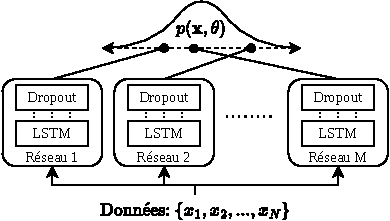
\includegraphics[width=0.85\linewidth]{Chapitre 1/Prono/Figures/mcdropout.pdf}
    \caption{Schéma de principe du Monte-Carlo \textit{dropout} pendant l'inférence - le \textit{dropout} est conservé et une étude statistique est possible sur les prédictions}
    \label{fig:mcdropout_principe}
\end{figure}
\FloatBarrier

\subsubsection{Intervalles de confiance pour le pronostic}

L'incertitude estimée par MC \textit{dropout} permet de définir un intervalle de
confiance empirique autour de la trajectoire de dégradation prédite.
Les intervalles sont ici calculés autour des prédictions de chaque instant en regardant les prédictions faites par toutes les passes avant :
 
\begin{equation}
    \mathcal{I}_t^{\alpha} =
    \left[
        Q_{\frac{1-\alpha}{2}}\!\left(\{\hat{y}_t^{(m)}\}\right),\;
        Q_{1-\frac{1-\alpha}{2}}\!\left(\{\hat{y}_t^{(m)}\}\right)
    \right]
    \label{eq:mcd_interval}
\end{equation}
 
où $Q_p$ désigne le quantile d'ordre $p$ calculé sur l'ensemble des $M$
prédictions et $\alpha$ est le niveau de confiance souhaité. Dans cette étude, $\alpha = 0.95$~: l'intervalle est délimité par les percentiles à \SI{2.5}{\percent} et \SI{97.5}{\percent} de l'ensemble des trajectoires MC. Contrairement à une approche paramétrique qui supposerait une distribution gaussienne des erreurs, les intervalles sont ici calculés directement par percentiles empiriques sur les $M$ trajectoires. L'intervalle de confiance s'élargit naturellement avec l'horizon de prédiction, traduisant la croissance de l'incertitude épistémique au fur et à mesure que le réseau extrapole au-delà des données observées.
Le calcul du RUL est ensuite réalisé en identifiant l'instant auquel la prédiction croise le seuil de fin de vie $\text{SoH}_{\text{EoL}}$.

% - - - - - - - - - - - - - - - - - - - - - - - - - - - - - -
\subsubsection{Application}
% - - - - - - - - - - - - - - - - - - - - - - - - - - - - - -

L'approche MC \textit{dropout} est appliquée de façon identique aux trois composants du micro-réseau~: batterie, PEMFC et PEMWE. Pour chaque composant, le réseau LSTM entraîné est utilisé en mode inférence avec \textit{dropout} actif pour générer $M = 500$ trajectoires de SoH sur un horizon de prédiction d'environ 165 jours. La moyenne de ces trajectoires constitue la prédiction centrale, et l'écart-type empirique la mesure d'incertitude associée. Les résultats sont présentés à la Figure~\ref{fig:mcdropout_results}, où une trajectoire d'état de santé artificielle avec une sinusoïde bruitée a été ajoutée pour évaluer la capacité de généralisation du réseau.

\begin{figure}[h!]
    \begin{minipage}{.33\linewidth}
    \centering
    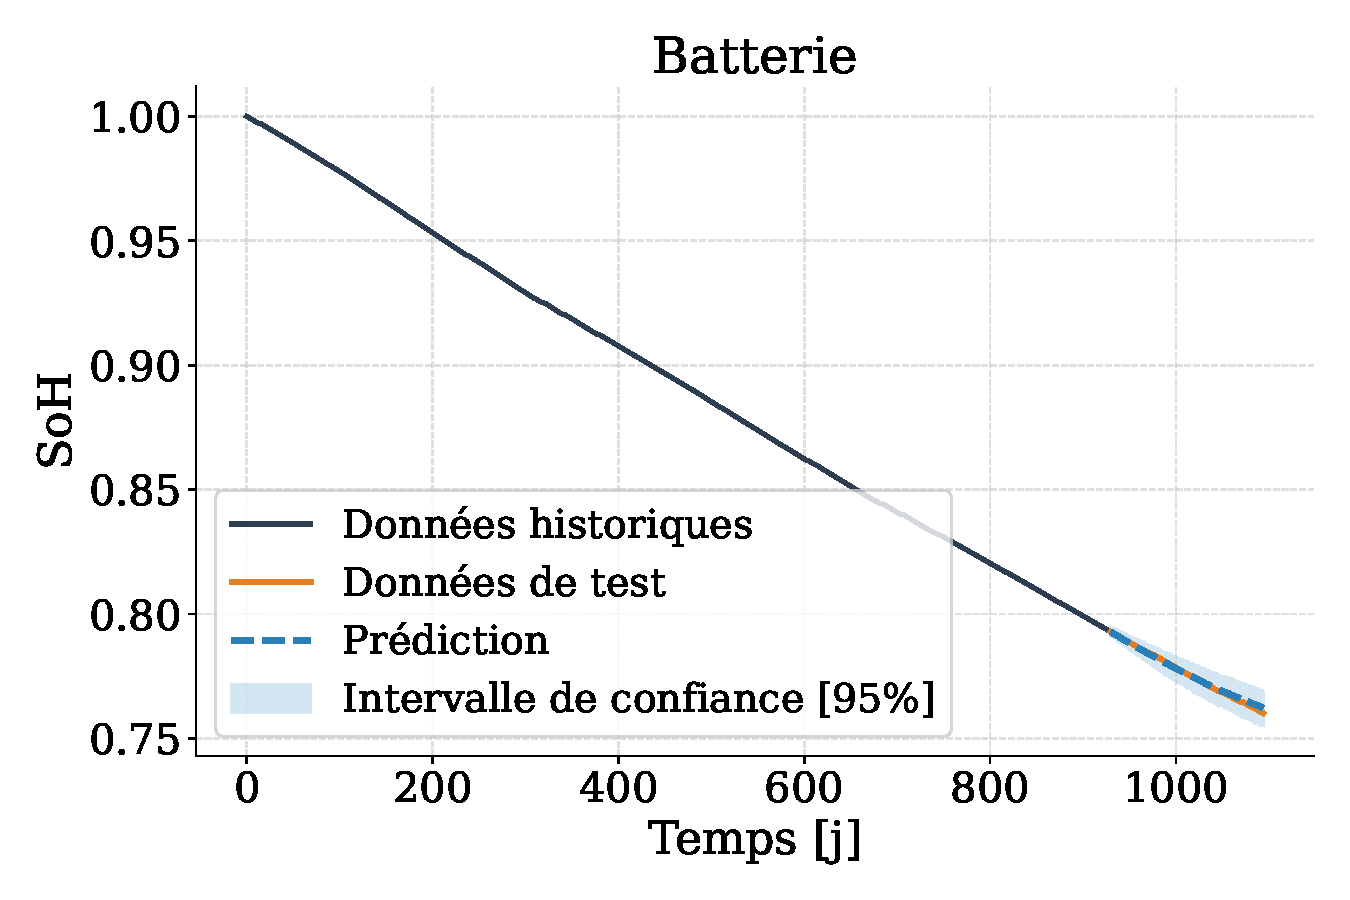
\includegraphics[width=\linewidth]{Chapitre 1/Prono/Figures/Batterie_trajectoire.pdf}
    \end{minipage}%
    \hfill
    \begin{minipage}{.33\linewidth}
    \centering
    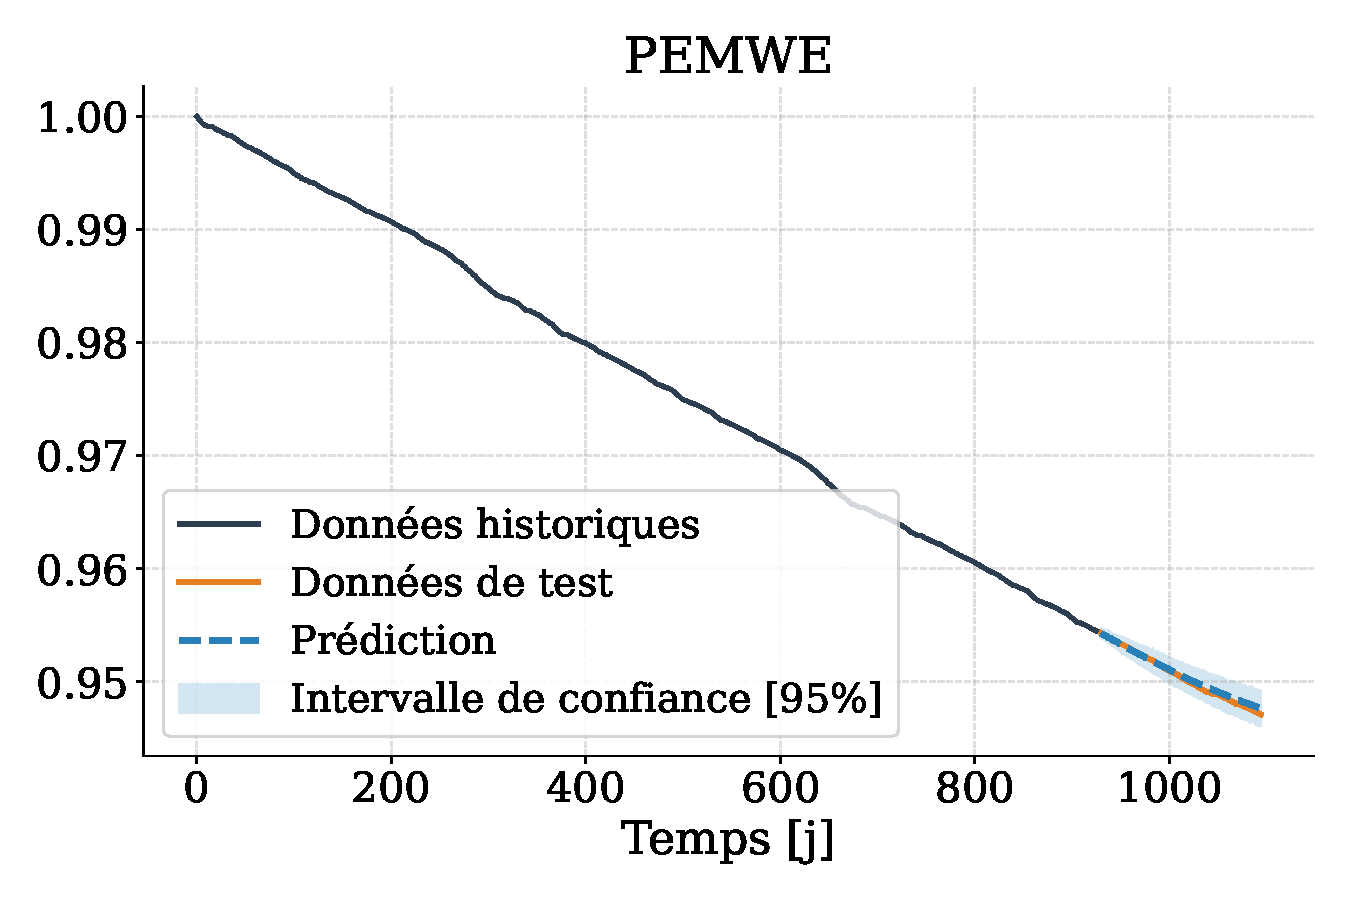
\includegraphics[width=\linewidth]{Chapitre 1/Prono/Figures/PEMWE_trajectoire.pdf}
    \end{minipage}
    \hfill
    \begin{minipage}{.33\linewidth}
    \centering
    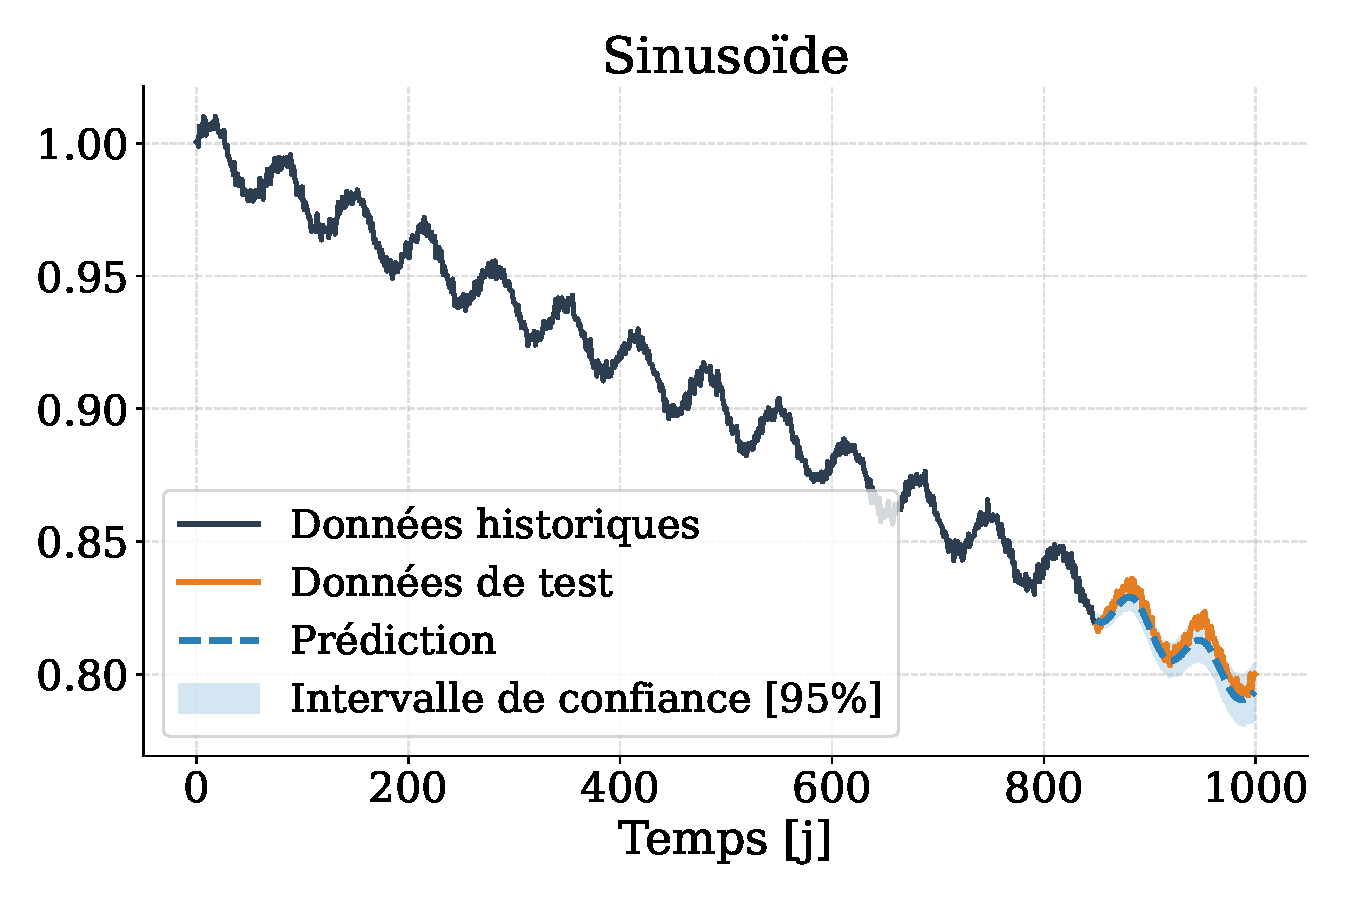
\includegraphics[width=\linewidth]{Chapitre 1/Prono/Figures/Sinusoïde_trajectoire.pdf}
    \end{minipage}
\end{figure}
\FloatBarrier
\begin{figure}[h!]
    \begin{minipage}{.33\linewidth}
    \centering
    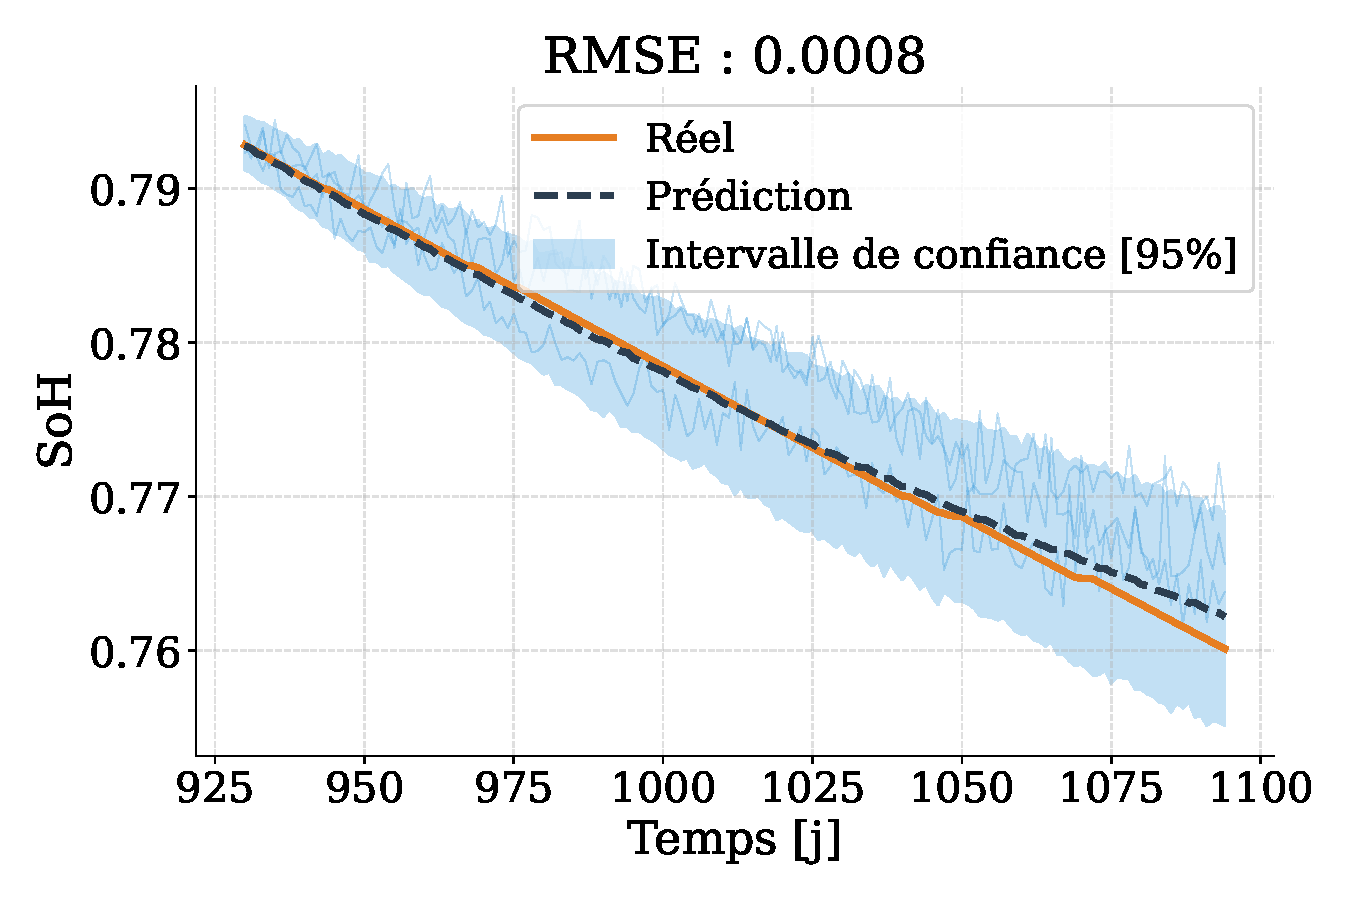
\includegraphics[width=\linewidth]{Chapitre 1/Prono/Figures/Batterie_zoom.pdf}
    \end{minipage}%
    \hfill
    \begin{minipage}{.33\linewidth}
    \centering
    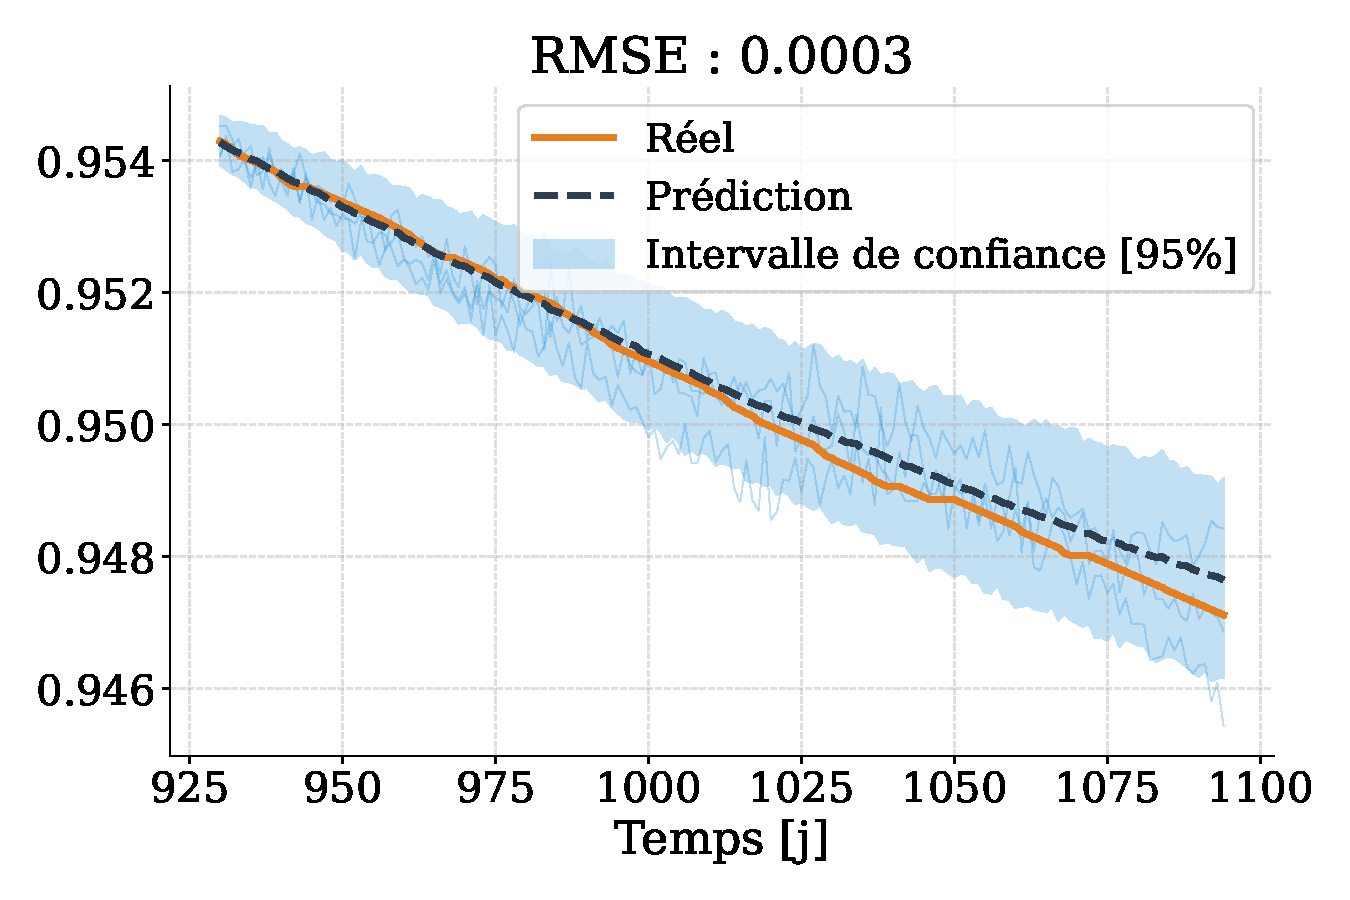
\includegraphics[width=\linewidth]{Chapitre 1/Prono/Figures/PEMWE_zoom.pdf}
    \end{minipage}
    \hfill
    \begin{minipage}{.33\linewidth}
    \centering
    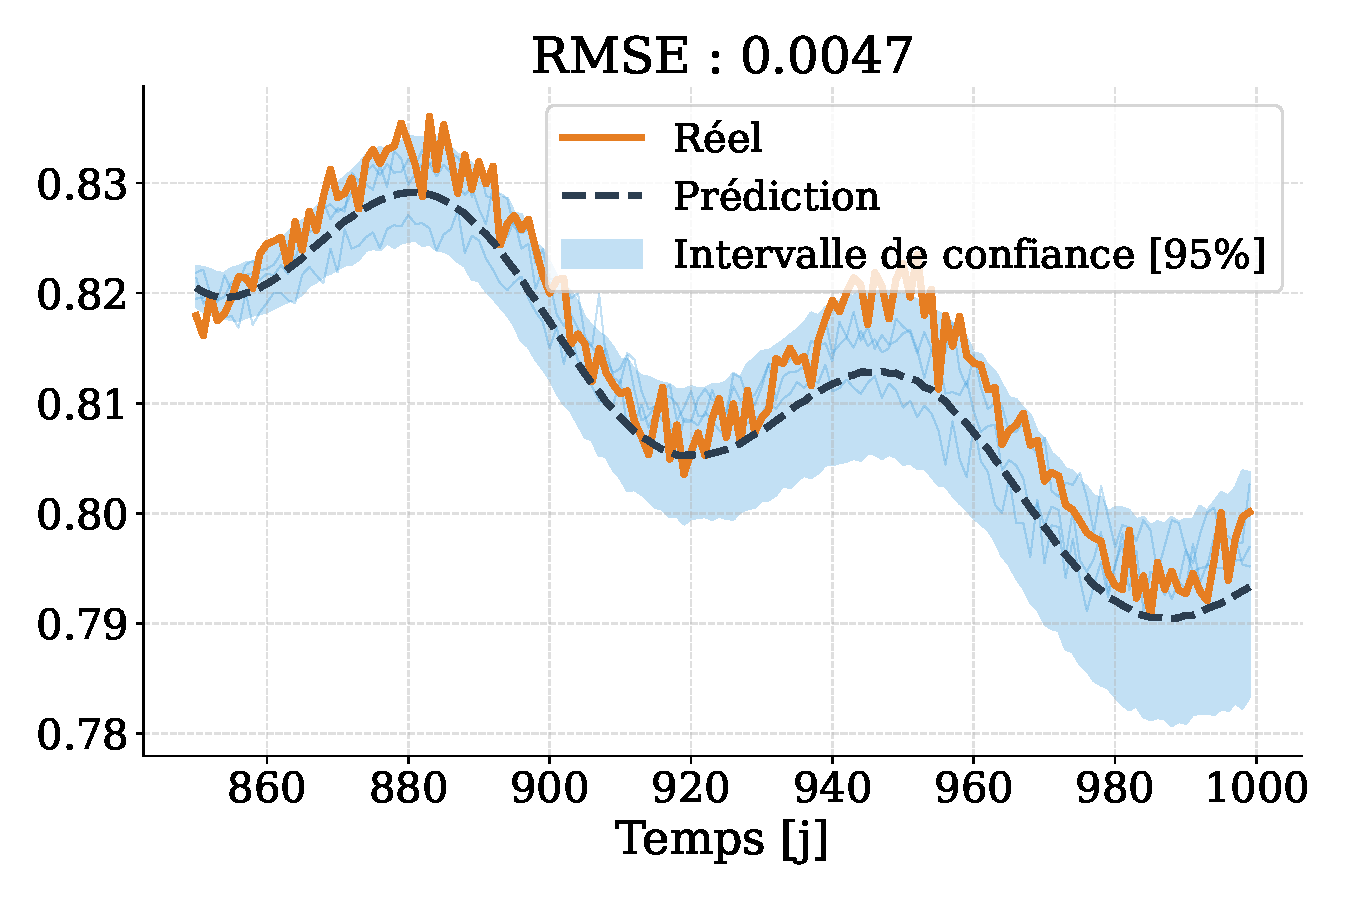
\includegraphics[width=\linewidth]{Chapitre 1/Prono/Figures/Sinusoïde_zoom.pdf}
    \end{minipage}
    \label{fig:mcdropout_results}
    \caption{Prédiction de l'évolution des états de santé des batteries (gauche), PEMWE (milieu) et une trajectoire sinusoïdale (droite) par Monte-Carlo \textit{dropout}}
\end{figure}
\FloatBarrier

L'intervalle de confiance obtenu s'élargit naturellement avec l'horizon de prédiction, traduisant la croissance de l'incertitude au fur et à mesure que le réseau extrapole au-delà des données observées. 
Le calcul du RUL est ensuite réalisé en identifiant l'instant auquel la prédiction d'état de santé croise le seuil de fin de vie $\text{SoH}_{\text{EoL}}$. Les bornes de l'intervalle de confiance donnent des estimations optimistes ou conservatrices du RUL (voir figure \ref{fig:rul_results}.)

\begin{figure}[h!]
    \centering
    % placeholder — calcul du RUL à partir des intervalles de confiance :
    % intersection borne basse vs seuil EoL, valeur centrale du RUL,
    % pour les trois composants
    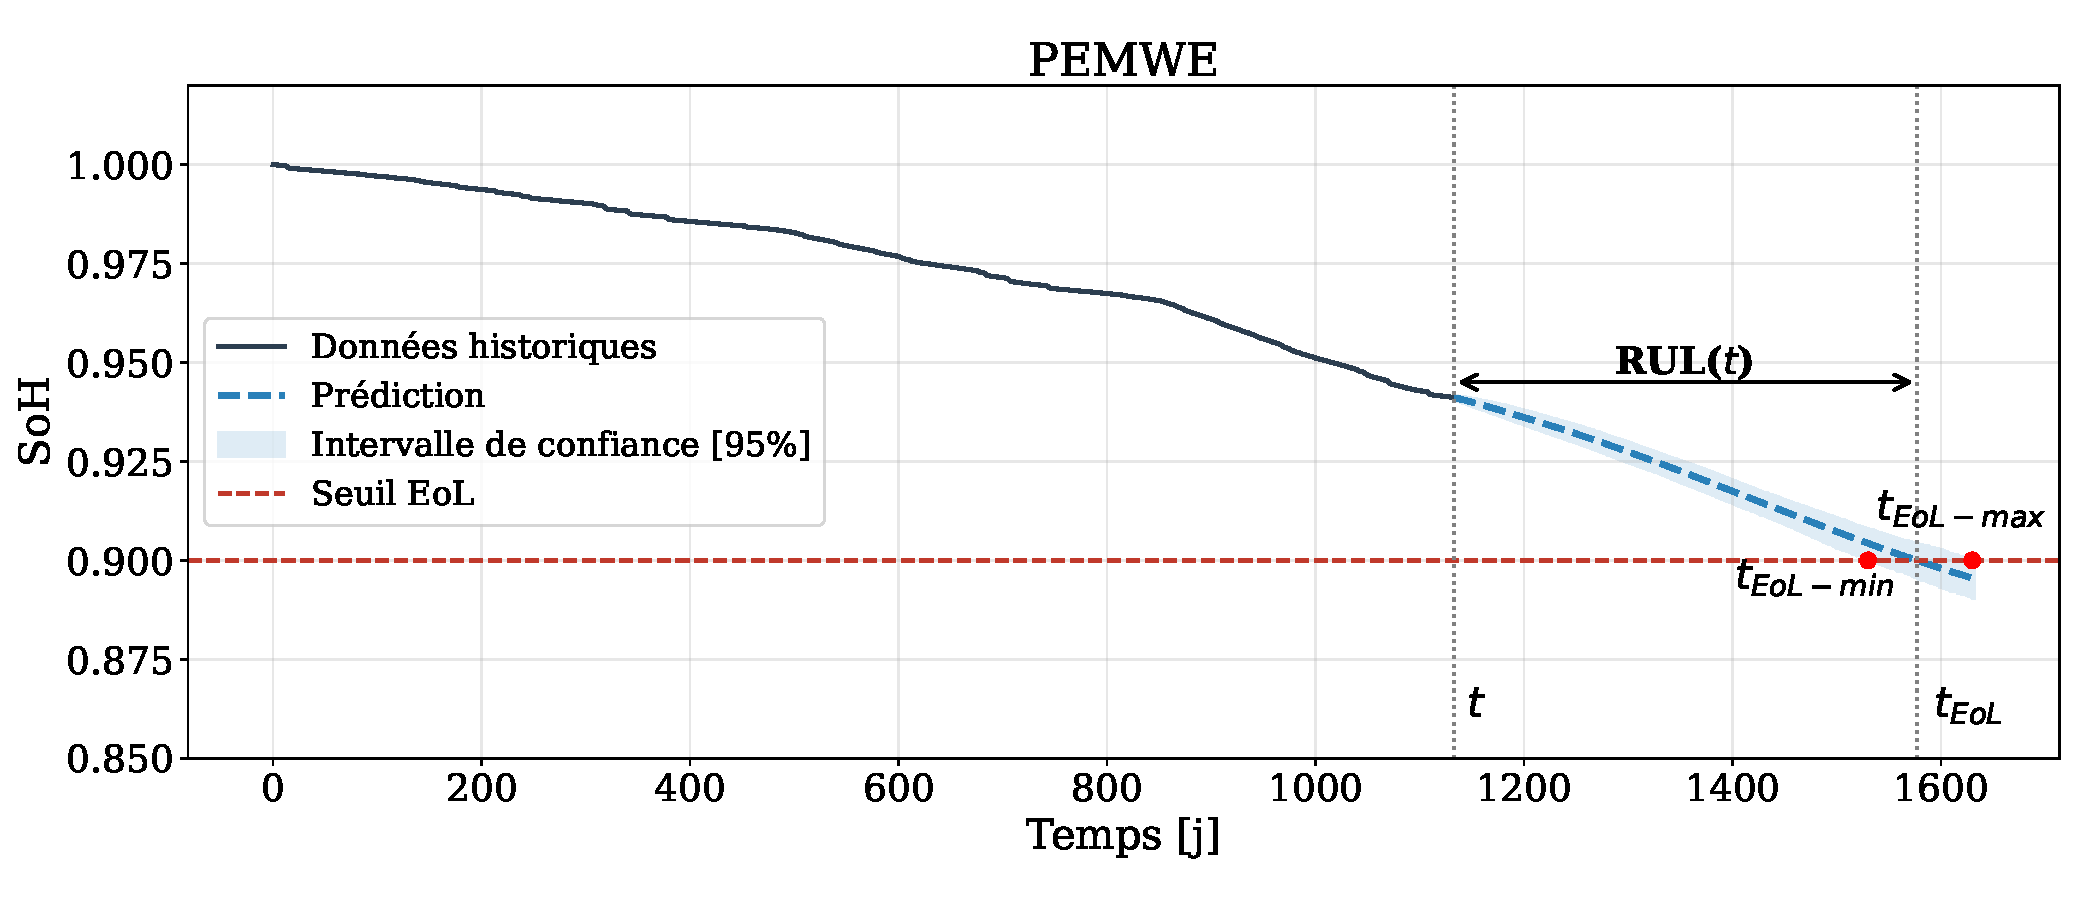
\includegraphics[width=\linewidth]{Chapitre 1/Prono/Figures/representation_rul_ely.pdf}
    \caption{Estimation du RUL du PEMWE, et représentation des bornes inférieures et supérieures des temps de fin de vie}
    \label{fig:rul_results}
\end{figure}
\FloatBarrier


\subsection{Discussion}
L'approche LSTM avec quantification d'incertitude par MC \textit{dropout} présente plusieurs avantages pour le pronostic de systèmes de stockage d'énergie. En premier lieu, l'architecture est entièrement basée sur les données~: aucune connaissance a priori sur les mécanismes physiques de dégradation n'est requise, ce qui garantit la capacité de généralisation de la méthode aux trois composants étudiés (batterie, PEMFC, PEMWE) malgré leurs mécanismes de vieillissement très
différents. Cela est confirme avec l'application du réseau sur un profil de nature très différente avec cette trajectoire sinusoïdale. En second lieu, l'estimation d'un intervalle de confiance autour de
la trajectoire de dégradation prédite apporte une information qualitative sur la fiabilité du pronostic, absente des méthodes ponctuelles classiques.
 
Il convient cependant de nuancer l'interprétation bayésienne du MC \textit{dropout}. Gal et Ghahramani~\cite{pmlr-v48-gal16} montrent que le \textit{dropout} à l'inférence constitue une approximation variationnelle d'un processus gaussien profond, et non une inférence bayésienne exacte. L'incertitude quantifiée est purement épistémique~: elle reflète l'incertitude sur les poids du réseau due à la quantité limitée de données d'entraînement, mais ne capture pas l'incertitude aléatoire inhérente au bruit de mesure du SoH ou à la variabilité des conditions d'utilisation. En pratique, cette distinction implique que les
intervalles de confiance peuvent être sous-estimés, notamment pour des profils de
dégradation s'écartant significativement de ceux observés à l'entraînement.
 
Il est attendu également que l'approche soit plus précise pour les composants dont la trajectoire de dégradation est régulière et quasi-linéaire. Les composants présentant des dynamiques de vieillissement non stationnaires ou des ruptures de pente (e.g., liées à des changements de régime d'exploitation) sont naturellement plus difficiles (voir impossible) à pronostiquer, et l'élargissement de l'intervalle de confiance traduit cette incertitude accrue.
 
Enfin, la stratégie de prédiction récursive implique une propagation de
l'erreur~: toute déviation entre la trajectoire prédite et la trajectoire réelle se répercute sur les pas suivants via l'auto-alimentation de la fenêtre. Cette propriété explique l'élargissement progressif des intervalles de confiance avec
l'horizon de prédiction. 

\subsection{Limitations}
Plusieurs limitations de l'approche proposée méritent d'être soulignées. Les séries de SoH utilisées sont issues d'un modèle de simulation et non de mesures expérimentales sur le micro-réseau réel de La Réunion. Les performances rapportées sont donc conditionnelles à la fidélité du modèle de simulation aux dynamiques de vieillissement réelles. 
 
Il est notable aussi que le réseau LSTM est entraîné sur une fenêtre temporelle fixe. Dans l'hypothèse où les conditions d'exploitation du micro-réseau évoluent sur l'horizon de la prédiction (changement de profil de charge, maintenance corrective, remplacement partiel), la stationnarité de la relation entrée--sortie apprise lors de l'entraînement n'est plus garantie. L'incertitude épistémique captée par le MC \textit{dropout} reflète l'incertitude sur les paramètres du modèle, mais pas cette non-stationnarité intrinsèque.
 
Comme discuté à la section précédente, l'approche MC \textit{dropout} ne quantifie que l'incertitude épistémique. L'incertitude aléatoire, liée au bruit de mesure et à la variabilité des conditions opérationnelles, n'est pas modélisée. Des approches telles que les réseaux bayésiens variationnels~\cite{kendall_what_2017} ou l'hétéroscédasticité apprise (\textit{learned aleatoric uncertainty}) permettraient de décomposer explicitement ces deux sources d'incertitude, au prix d'une complexité d'implémentation et de coût de calcul plus élevés.
 
Finalement, l'architecture retenue (association d'une couche LSTM, d'une couche de \textit{dropout} et une couche dense) peut ne pas être optimale. Des architectures plus profondes ou des variantes bidirectionnelles pourraient améliorer la précision de la prédiction centrale, mais compliqueraient également l'interprétation bayésienne du MC \textit{dropout}. Ce point constitue une piste d'amélioration future pour les travaux de pronostic sur les composants de stockage d'énergie.

\newpage